\Introduction

Система состоит из трех независимых элементов, соединенных последовательно с точки зрения надежности. Плотности распределения времени безотказной работы заданы графически при $0<t<1$, см.~Рис.~\ref{img:10-0}

\begin{figure}[h]
  \centering
  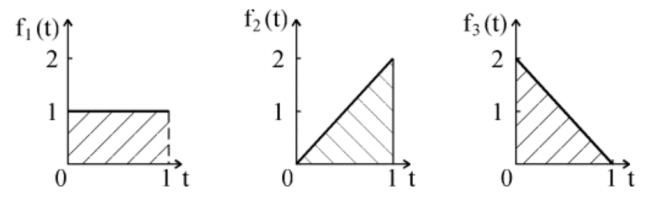
\includegraphics[width=.9\linewidth]{assets/baseConnect}
  \caption{Плотностб вероятности $f_{1}$, $f_{2}$, $f_{3}$}
  \label{img:10-0}
\end{figure}

Найдите интенсивность отказов системы как функцию времени на наработке $0 < t < 1$. Постройте графики $\lambda_{1}$, $\lambda_{2}$, $\lambda_{3}$, $\lambda_{sys}$.
